\documentclass{article}
\usepackage[utf8]{inputenc}
\usepackage[T1]{fontenc} 
%\usepackage[french]{babel}
\usepackage{charter} 
\usepackage{graphicx} 
\usepackage{amsmath}
\usepackage{amsthm}
\usepackage{amsfonts}
\usepackage{geometry}
\usepackage{cancel}
\usepackage{enumerate}
\usepackage{stmaryrd}
\usepackage{mathrsfs}
\usepackage{amssymb}
\geometry{hmargin=2.7cm,vmargin=2.5cm}

\usepackage{lastpage}
\usepackage{fancyhdr}
\pagestyle{fancy}
\renewcommand{\headrulewidth}{0pt}
\renewcommand{\footrulewidth}{0.5pt}
\fancyhead[L]{}
\fancyhead[R]{}
\fancyfoot{}
\fancyfoot[L]{RS -- Quentin CHAN-WAI-NAM}
\fancyfoot[R]{\thepage/\pageref{LastPage}}

\fancypagestyle{plain}{
	\renewcommand{\headrulewidth}{0pt}
	\renewcommand{\footrulewidth}{0.5pt}
	\fancyhead[L]{}
	\fancyhead[R]{}
	\fancyfoot{}
	\fancyfoot[L]{RS -- Quentin CHAN-WAI-NAM}
	\fancyfoot[R]{\thepage/\pageref{LastPage}}
}

\def\thesubsection{\thesection.\alph{subsection}}

\makeatletter
\def\thm@space@setup{%
  \thm@preskip=15pt \thm@postskip=15pt
}
\makeatother

\linespread{1.3}

\newcommand{\abs} [1] {\left| #1 \right|}
\newcommand{\scal}[2]{\left\langle #1 , #2 \right\rangle}
\newcommand{\dif}[0]{\text{\:d}}
\newcommand{\Dpar}[2]{\frac{\partial#1}{\partial#2}}

\newcommand{\ceil}[1]{\lceil#1\rceil}
\newcommand{\floor}[1]{\lfloor#1\rfloor}

\newcommand{\Four}[1]{\widehat{#1}}

\newcommand{\norm}[1]{\left\lVert#1\right\rVert}

\def\R{\mathbb{R}}
\def\Z{\mathbb{Z}}
\def\N{\mathbb{N}}
\def\e{\text{e}}
\def\d{\text{d}}
\def\Re{\text{Re}}

\def\Per{\text{Per}\,}
\def\Ker{\text{Ker}\,}
\def\Im{\text{Im}\,}

\def\Ind{\mathbf{1}}

% Width of the EPIs
\def\epiWidth{0.8}

\newcommand{\Binom}[2]{\begin{pmatrix} #1 \\ #2 \end{pmatrix}}

\newcommand{\vect}[1]{\mathbf{#1}}

%%%%%%%%%%%%%%%%%%%%%%%%%%%%%%%%%%%%%%%%%%%%%%%%%%%%%%%%%%%%%%%%%%%%%%%%%%%%%%%%%%%%%%%%%%%%%%%%

\title{RS: Epipolar Plane Image Analysis\\Application to SkySat videos}
\date{\today}
\author{Quentin CHAN-WAI-NAM}

\theoremstyle{definition}
\newtheorem{question}{}

\begin{document}
\maketitle


\section{Choice of the article and objective}


We first investigated two different articles that describe two different methods for estimating depths maps from videos.
\begin{itemize}
 \item \cite{art:perez13:tvl1} describes an algorithm that estimates the optical flow given two images using a global optimization scheme minimizing a data attachment term and a regularization using the total variation of the flow. The idea is that the brightness $I$ of single points along their trajectories should be constant in time, leading to the optical flow constraint equation
 \[ \nabla I \cdot \vect{u} + \Dpar{I}{t} = 0 \]
 where $\vect{u}$ is the optical flow (the velocity vector field). The article then introduces a regularization on $\vect{u}$ (its total variation) and reformulates the problem in order to adapt to discrete sequences of images so that the attachent term consists in minimizing some $L^1$ term. In order to solve the subsequent global optimization problem, the authors propose a numerical scheme based on alternate optimization scheme. Finally, the authors investigate the influence of the several parameters of the algorithm -- noticeably the weight $\lambda$ of the data attachment term -- on the precision of the estimation of the optical flow and the sensitivity to noise.
 
 In our case, the optical flow computed with this algorithm could be interpreted as some disparity measurement. An interesting point is that the computation of the optical flow can be done on any pair of images, even if not rectified.
 
 \item \cite{art:kim13:lfields} describes a method for computing precise and exhaustive depth maps using ``light fields'', that is a dense set of images captures along a linear path. By concatenating one line of the rectified images together, one obtains an ``epipolar-plane image'' (EPI), in which a single scene point appears as a linear trace which slope is related to its distance to the camera. Thus, by estimating these slopes, one can reconstruct the depth of each point of the scene.
 
 The authors use very high definition images, so that the article includes several implementation details in order to ensure computational feasibility, both in terms of space (sparse representation of light fields) and computational power. For instance, they prefer local optimization near object boundaries and propagation to nearby areas in a fine-to-coarse approach to global optimization on the whole image. In the end, the method seems relatively fast, precise and robust to inconsistencies and outliers like noise or temporary occlusions.
\end{itemize}


We chose to work on the latter article. The objective of the project is then to implement the method presented by Kim et al. in \cite{art:kim13:lfields} and investigate how it performs with videos taken from SkySat. We will first investigate the case in which the images from the video are pre-rectified. Then we will investigate more complicated situations, for instance increasing the density of the images and considering non-pre-rectified sequences.


\section{Sample EPIs from Skysat (step 18)}


\paragraph{Test} \verb#test_build_row_epi_skysat_rectified_18.cpp#.


We first write codes to compute and display EPIs. We investigate possible artefacts that appear in the EPIs extracted from the rectified images of Skysat, with step $18$.


\begin{figure}[ht]
  \centering
  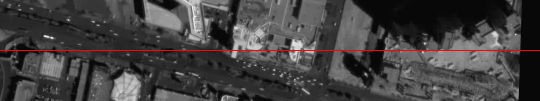
\includegraphics[width=\epiWidth\textwidth]{images/1519991014186_1st.png}\\
  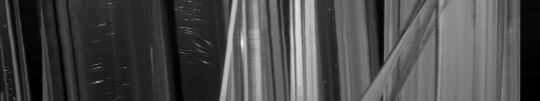
\includegraphics[width=\epiWidth\textwidth]{images/1519991014186_epi.png}
  \caption{Row 600 -- We can see that the cars produce some artefacts.}
\end{figure}


\begin{figure}[ht]
  \centering
  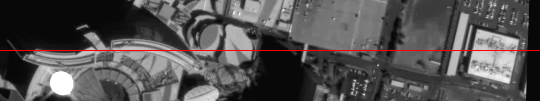
\includegraphics[width=\epiWidth\textwidth]{images/1519991030012_1st.png}\\
  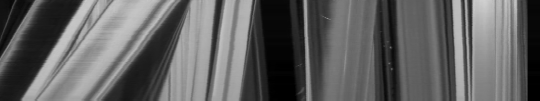
\includegraphics[width=\epiWidth\textwidth]{images/1519991030012_epi.png}
  \caption{Row 380 -- The high building has a very steep slope. The color of some points seem to vary in time (due to changes in illumination and shading). We also note some strong occlusions.}
\end{figure}


\begin{figure}[ht]
  \centering
  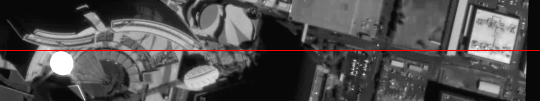
\includegraphics[width=\epiWidth\textwidth]{images/1519991772641_1st.png}\\
  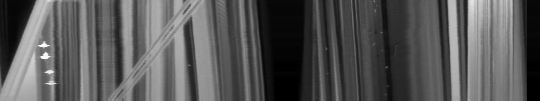
\includegraphics[width=\epiWidth\textwidth]{images/1519991772641_epi.png}
  \caption{Row 400 -- The specular reflexions produce artefacts.}
\end{figure}


\begin{figure}[ht]
  \centering
  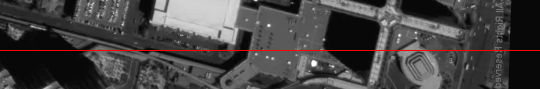
\includegraphics[width=\epiWidth\textwidth]{images/1519992108606_1st.png}\\
  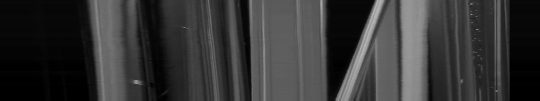
\includegraphics[width=\epiWidth\textwidth]{images/1519992108606_epi.png}
  \caption{Row 920 -- The shadows produce empty black zones.}
\end{figure}


\section{First rough estimation of the disparities}


\paragraph{Principle} We apply a very simplified version of the first step of the ``fine to coarse'' approach of \cite{art:kim13:lfields}: we take some EPI $E$ corresponding to a fixed $v$, which dimensions are $S$ along the rows and $U$ along the columns. We work only on one line of this EPI (the center line, at $\widehat{s} = S / 2$. Let $d_\text{list} = \left\{d_1, \cdots, d_D \right\}$ be a search set of disparities. We compute the set of radiances $\mathcal{R}$ for all couples $(u, d)$:
\[ \mathcal{R}(u, d) = \left\{ E(u + (\widehat{s} - s) d, s) \; | \; s = 0 \cdots S-1 \right\}. \]

We then compute a score $S(u, d)$ defined as:
\[ S(u, d) = \frac{1}{\abs{\mathcal{R}(u, d)}} \sum_{\mathbf{r} \in \mathcal{R}(u, d)} K(\mathbf{r} - \overline{\mathbf{r}})\]
where $\mathbf{r}$ can be a float, or in the case of the images of the mansion, a tricolor vector, and $K$ is a ``kernel''. We choose the kernel presented in the article, i.e.
\[ K(\mathbf{r}) = \left\{ 
\begin{array}{l}
1 - \norm{\mathbf{r} / h}^2 \qquad \text{if $\norm{\mathbf{r} / h} < 1$} \\
0 \qquad \text{else}                            
\end{array} \right. .
\]
We name this kernel the ``bandwidth kernel'' (and we take $h = 0.2$ arbitrarily for now).

$\overline{\mathbf{r}}$ is a parameter that depends on $(u, d)$: following the article, we perform a truncated mean-shift algorithm (10 iterations), with $\overline{\mathbf{r}}_0 = E(u, \widehat{s})$ and
\[ \overline{\mathbf{r}} \leftarrow \frac{\sum_{\mathbf{r} \in \mathcal{R}(u, d)} K(\mathbf{r} - \overline{\mathbf{r}}) \mathbf{r}}{\sum_{\mathbf{r} \in \mathcal{R}(u, d)} K(\mathbf{r} - \overline{\mathbf{r}})}\]
prior to the computation of $S(u, d)$.

Finally, for each $u$, we select the $d$ with the best score. We discard scores $< 0.01$ ; if no score is available, then we take $d=0$. We apply a linear median filter (along the $u$ dimension only for now) on the resulting values $d$ (we choose a filter size of $5$).

We propagate the disparities from $\widehat{s}$ to the other $s$ simply by drawing the depths along the lines $u + (\widehat{s} - s)d$ and respecting the occlusions (a point with higher disparity will be ``occluding'' a point with a lesser disparity).


\paragraph{Technical difficulties} A line defined by $(u + (\widehat{s} - s) d, s)$ will very certainly end up going out of the image. Moreover, these coordinates are not integer coordinates. We thus take the following decisions:
\begin{itemize}
 \item Values outside of the image are considered \emph{nan} and not taken into account in $\mathcal{R}(u, d)$.
 \item We have yet to decide on some proper interpolation method for computing non-integer values of $E$. For now, we choose a simple linear interpolation along the line $E(u, \cdot)$.
 \item The complexity of the algorithm increases quite a bit with the dimensions of the image. We might implement the algorithms using GPUs, but now we use tricks like OpenMP.
\end{itemize}
We also created a template code so as to be able to adapt to different data types for $E$ (e.g. \verb#float#, \verb#uint#, \verb#cv::Vec3b#...).


\paragraph{Results} We choose $d_\text{list} = \left\{-2.0, -2.05, \cdots, 3.95, 4.0\right\}$. We end up with the following results. We expect to improve these using confidence scores $C_e$ as in the article for instance, and computing depths for more $s$ than only $\widehat{s}$.


\begin{figure}[ht]
  \centering
  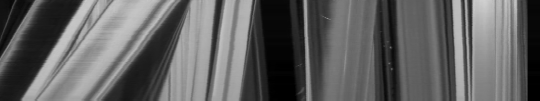
\includegraphics[width=\epiWidth\textwidth]{images/1520204861279_epi.png}\\
  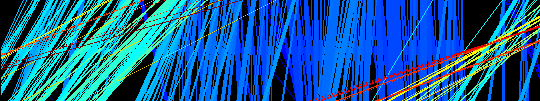
\includegraphics[width=\epiWidth\textwidth]{images/1520204861279_epi_colored.png}
  \caption{Skysat rectified, row 380. We note some parasite extreme lines. We interpret these as parasite low-confidence slopes.}
\end{figure}


\begin{figure}[ht]
  \centering
  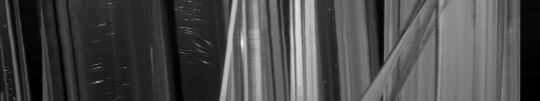
\includegraphics[width=\epiWidth\textwidth]{images/1520205010590_epi.png}\\
  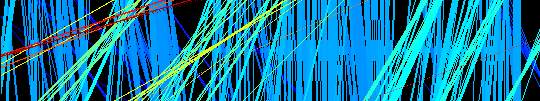
\includegraphics[width=\epiWidth\textwidth]{images/1520205010590_epi_colored.png}
  \caption{Skysat rectified, row 600. Cars do not seem to make a huge difference, but homogeneous zones are not well handled.}
\end{figure}


\begin{figure}[ht]
  \centering
  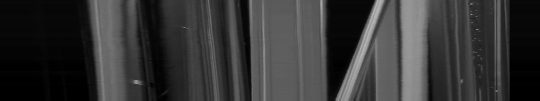
\includegraphics[width=\epiWidth\textwidth]{images/1520205074004_epi.png}\\
  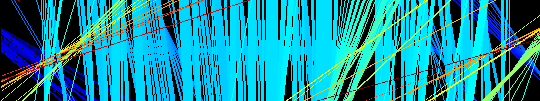
\includegraphics[width=\epiWidth\textwidth]{images/1520205074004_epi_colored.png}
  \caption{Skysat rectified, row 920. As expected, the algorithm does not work well in the shadows.}
\end{figure}


\begin{figure}[ht]
  \centering
  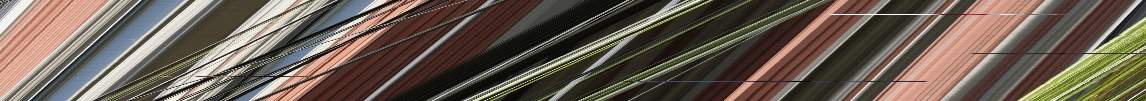
\includegraphics[width=\epiWidth\textwidth]{images/1520202945623_epi.png}\\
  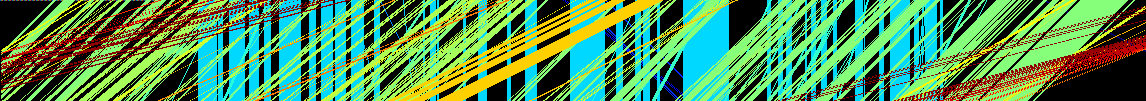
\includegraphics[width=\epiWidth\textwidth]{images/1520202945623_epi_colored.png}
  \caption{Mansion sample (undersized to $1146\times 720$), row 380.}
\end{figure}


\section{After scaling}


In fact, it is better to scale the images between $0.0$ and $1.0$ before processing. We do the following:
\begin{itemize}
 \item If the provided image is of type \verb#uchar#, i.e. values are in $0 \cdots 255$, then we scale by $255$.
 \item Else, we scale by the max over all the channels.
\end{itemize}
Results are much cleaner:


\begin{figure}[ht]
  \centering
  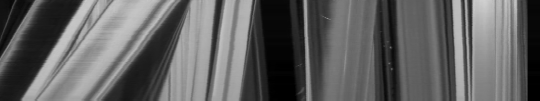
\includegraphics[width=\epiWidth\textwidth]{images/1520334265034_epi.png}\\
  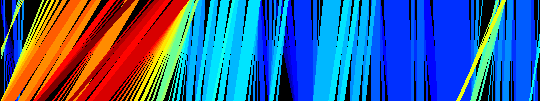
\includegraphics[width=\epiWidth\textwidth]{images/1520334265034_epi_colored.png}
  \caption{Skysat rectified, row 380.}
\end{figure}


\begin{figure}[ht]
  \centering
  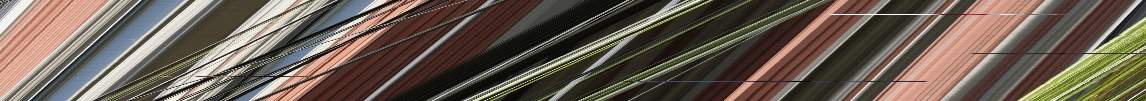
\includegraphics[width=\epiWidth\textwidth]{images/1520334290628_epi.png}\\
  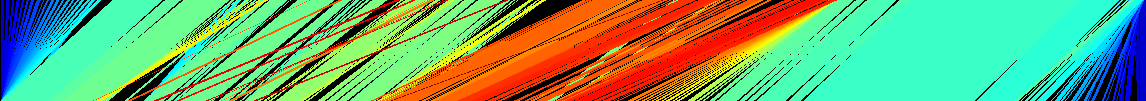
\includegraphics[width=\epiWidth\textwidth]{images/1520334290628_epi_colored.png}
  \caption{Mansion sample (undersized to $1146\times 720$), row 380.}
\end{figure}


\clearpage
\bibliographystyle{plain}
\bibliography{bibliography}


\end{document}